\documentclass{scrartcl}
\usepackage{graphicx}
\usepackage{subcaption}
\usepackage{graphics}

\usepackage{listings}
\usepackage{color}

\renewcommand\lstlistingname{Quelltext} % Change language of section name

\lstset{ % General setup for the package
language=Python,
basicstyle=\small\sffamily,
numbers=left,
numberstyle=\tiny,
frame=tb,
tabsize=4,
columns=fixed,
showstringspaces=false,
showtabs=false,
keepspaces,
commentstyle=\color{red},
keywordstyle=\color{blue}
}

\makeatletter
\renewcommand\subparagraph{%
\@startsection {subparagraph}{5}{\z@ }{3.25ex \@plus 1ex
\@minus .2ex}{-1em}{\normalfont \normalsize \bfseries }}%
\makeatother

\begin{document}

\title{Activity Recognition}
\subtitle{Final project for Vision and Perception by Prof. Fiora Pirri}
\author{Son Tung Nguyen - Wei Xu - Zijian Xue}

\maketitle

\section{Introduction}
Activity recognition has been a fundamental problem in computer vision \cite{a1}.
Huge progress has been achieved with the success of convolutional neural network
(CNN) on image recognition or object detection tasks. In this work, we study
different solutions to recognize and organize human activities into multiple
categories. To be precise, our goal is to classify accurately a given video into
one of ten categories of housework activities.
\section{Related works}
Human activity recognition is a well studied problem. Some of the past works on
this topic include training support vector machine classifiers on bag-of-words
features \cite{a2, a3}. A more recent solution is to train a CNN to capture spatial
information and to use a long short term memory (LSTM) network to exploit temporal
features of videos. \cite{a1} was one of the first examples on this idea. Their works
showed that the proposed system performed very well on three different problems:
activity recognition, image captioning and video description.


\section{Proposed method}

\subsection{Model architecture}
Our model architecture follows the work of \cite{a1}. Figure 1 illustrates the standard architecture
of our system. For each frame, we have a CNN model to output spatial
features. This CNN model was pretrained on Imagenet and kept untrainable during
our training. The output of the CNN layer is forwarded to the LSTM layer to capture
temporal relationship of frames. After this, we calculate the softmax probabilities
of each frame and then output the average as our final prediction.

\subsection{Improvements}
We carried on multiple experiments on different ideas to enhance the ability of
the system.
\subparagraph{VGG-16 or Inception pretrained weights}
We had two options for the pretrained CNN layer: VGG-16 \cite{a6} or Inception V3 \cite{a7}. So,
we decided to try both. The result was as expected when using Inception V3
weights resulted in better performance (Table 1).
\subparagraph{Longer sequence}
Different video sequence was also tried. Experiments showed that using longer
sequence made the system better (Table 1).
\subparagraph{More LSTM layers}
Stacking more LSTM layers typically enhanced the performance of the system.
We tried to stack our system with 1, 2 and 3 layers and found that stacking resulted
in higher accuracy.
\subparagraph{Linear interpolating}
We tried to linear interpolate the loss function as suggested by \cite{a4}. To
be more exact, we weighted our loss function so that the model focuses more on
later time steps in the sequence. This is an alternative to just sum up the
softmax loss of every time steps.
\subparagraph{Exploit spatial information from object detection model}
We attempted to inject spatial information from a Mask-RCNN \cite{a8} model on every
frame into our system. That is, for every frame, we ran inference by Mask-RCNN
model and returned three vectors: $mask$, $bbox$ and $prob$. Each vector is
$T$-length depicted a pre-defined set of $T$ objects. The $mask$ and $bbox$ vectors
described the mask and bounding box areas of $T$ objects. The $prob$ vector
described the probabilities of detecting these $T$ objects. Figure 2 illustrates
an example of this architecture.

\section{Experiments}
\subparagraph{Datasets}
We used a subset of ActivityNet \cite{a5} as our data source for training and testing.
For each video, we extracted video segment that contains interested activities.
Each video segment is at most 10 second long. In the end, we had 856 video segments and
split them into train set of 680 segments and test set of 176 segments.
\subparagraph{Training settings}
To optimize our network, we used Adam optimization \cite{a9} with learning rate of $0.1$.
Each experiment was optimized for 100 epochs. Figure 3 shows the training profile
of our network and suggests that the model suffered from over-fitting.


\newpage
\begin{figure}[h!]
\centering
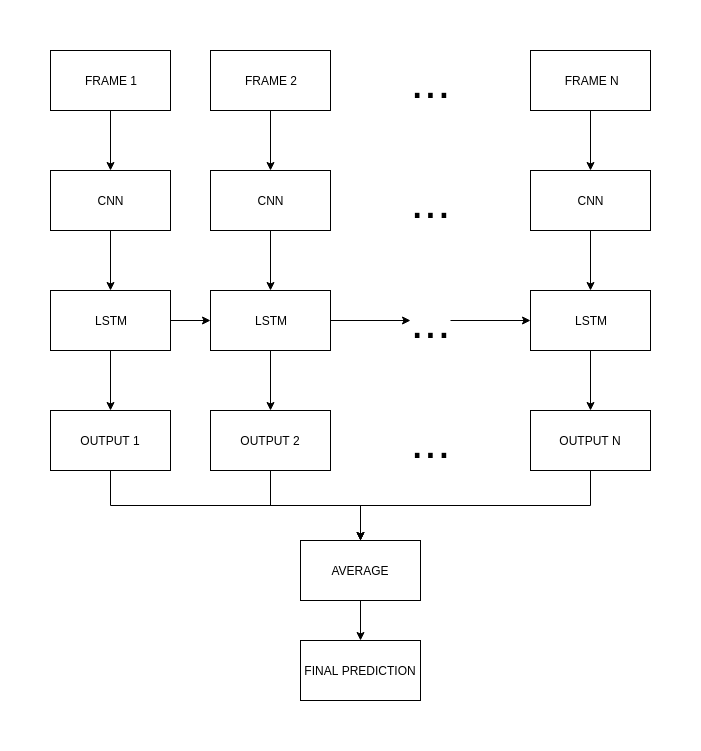
\includegraphics[width=400]{figures/model_standard.png}
\caption{Standard model architecture.}
\label{fig:1}
\end{figure}

\begin{figure}[h!]
\centering
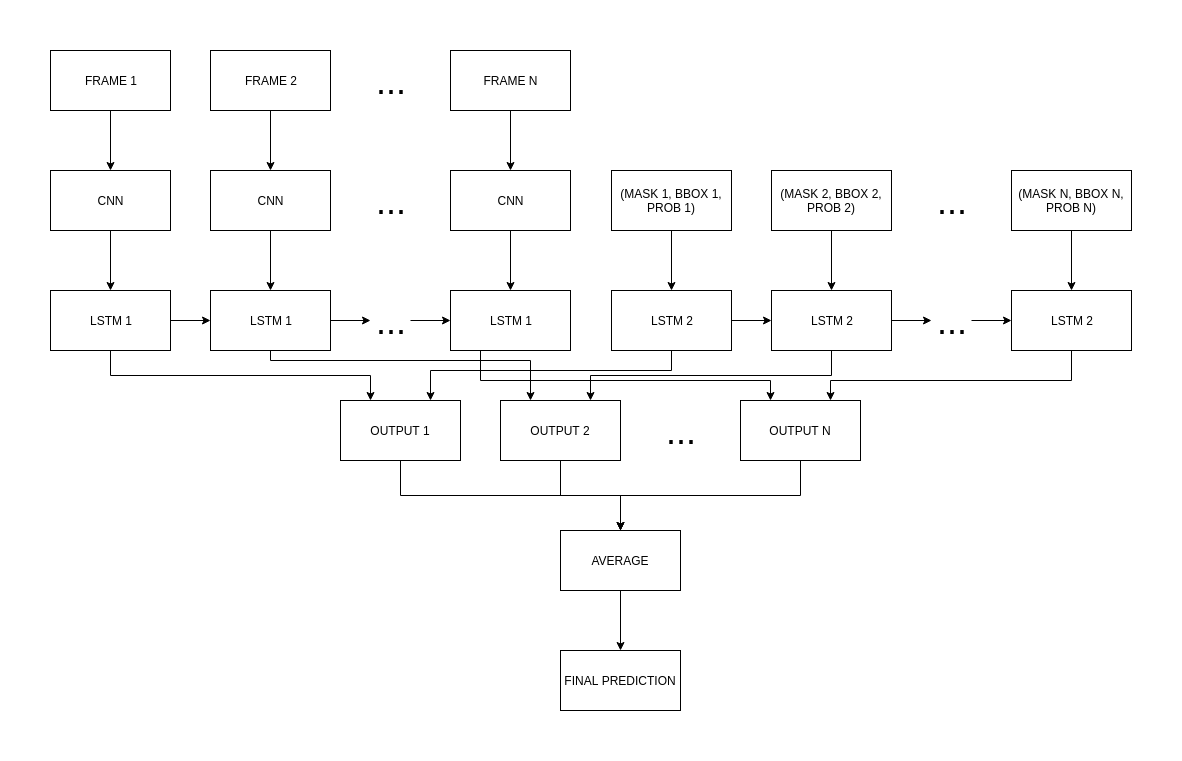
\includegraphics[width=400]{figures/model_2.png}
\caption{Model architecture that exploits spatial information from object detector.}
\label{fig:2}
\end{figure}

\begin{figure}[h!]
\centering

\includegraphics[width=400]{figures/train_profile.png}
\caption{Training profile with 4 LSTM layers.}
\label{fig:2}
\end{figure}

\begin{table}[h!]
\begin{center}
\caption{Pretrained weights and longer sequence.}
\label{t1}
\resizebox{\columnwidth}{!}{
\begin{tabular}{l|c|c|c|c|c|c|c|c}
\textbf{Pretrained weights} & \textbf{25} & \textbf{50} & \textbf{100}\\
\hline
VGG-16 & 0.447 & 0.494 & 0.484\\
Inception V3 & 0.546 & 0.557 & 0.593\\
\end{tabular}
}
\end{center}
\end{table}

\begin{table}[h!]
\begin{center}
\caption{Stacking different numbers of LSTM layers.}
\label{t1}
\resizebox{\columnwidth}{!}{
\begin{tabular}{l|c|c|c|c|c|c|c|c}
\textbf{} & \textbf{1} & \textbf{2} & \textbf{3} & \textbf{4} & \textbf{5}\\
\hline
Accuracy & 0.536 & 0.531 & 0.557 & 0.562 & 0.552\\
\end{tabular}
}
\end{center}
\end{table}

\begin{table}[h!]
\begin{center}
\caption{Using additional spatial information.}
\label{t1}
\resizebox{\columnwidth}{!}{
\begin{tabular}{l|c|c|c|c|c|c|c|c}
\textbf{Using prob} & \textbf{Using mask} & \textbf{Using bbox} & \textbf{Accuracy}\\
\hline
1 & 0 & 0 & 0.557\\
0 & 0 & 1 & 0.567\\
0 & 1 & 0 & 0.562\\
1 & 1 & 1 & 0.531\\
\end{tabular}
}
\end{center}
\end{table}



\clearpage
\bibliography{ref}
\bibliographystyle{ieeetr}

\end{document}
